\documentclass[12pt]{article}

\pagestyle{plain}
\textwidth 6.5 in
\oddsidemargin 0 in
\evensidemargin 0 in
\topmargin 0 in
\textheight 8 in

\pagestyle{empty}

\usepackage[all]{xy}
\usepackage{graphicx}
\usepackage{svg}
\usepackage{units}
\usepackage{enumerate}
\usepackage[hidelinks]{hyperref}
\usepackage[T1]{fontenc}
\usepackage{float}


\usepackage{amssymb, amsmath, pict2e}
 \pagestyle{myheadings}

\usepackage{pdfsync}
\usepackage{rotating}
\usepackage{multirow}
\usepackage[normalem]{ulem}
\usepackage{cancel}

\usepackage{color}
\usepackage{optidef} %formules d'optimisation 
\usepackage[usenames,dvipsnames,svgnames,table]{xcolor}
\usepackage{tikz}
\usetikzlibrary{arrows}
\usepackage{environ}
\usepackage{environ}
\makeatletter
\newsavebox{\measure@tikzpicture}
\NewEnviron{scaletikzpicturetowidth}[1]{%
  \def\tikz@width{#1}%
  \def\tikzscale{1}\begin{lrbox}{\measure@tikzpicture}%
  \BODY
  \end{lrbox}%
  \pgfmathparse{#1/\wd\measure@tikzpicture}%
  \edef\tikzscale{\pgfmathresult}%
  \BODY
}


\title{Reconfiguration problems\\
\small MEMO-F403 -- Preparatory work for the master thesis}


\author{Prateeba Ruggoo$^1$  \\  Department of Computer
Science \\ Universite Libre de Bruxelles\\ {\small pruggoo@ulb.ac.be$^1$}\\[0.5cm]{\small Advisor:
Jean Cardinal}}


\date{May 27, 2019}

%%%%%%%%%%%%%%%%  start macros  %%%%%%%%%%%%%%%%%%%%%%%%%%%%%%%%%
\newtheorem{theorem}{Theorem}
\newtheorem{defn}[theorem]{Definition}
\newtheorem{example}[theorem]{Example}
\newtheorem{remark}[theorem]{Remark}
\newtheorem{question}[theorem]{Question}

\newtheorem{lemma}[theorem]{Lemma}
\newtheorem{claim}[theorem]{Claim}
\newtheorem{prop}[theorem]{Proposition}
\newtheorem{corollary}[theorem]{Corollary}
\newtheorem{conjecture}[theorem]{Conjecture}

\newtheorem{hyp}[theorem]{Hypothesis}
\newtheorem{alg}[theorem]{Algorithm}
\numberwithin{theorem}{subsection}

\newcommand{\qed}{\mbox{$\Box$}}
\newcommand{\proof}{\medbreak\par\noindent{\bf Proof. }}
 \newcommand{\GP}{{\vec{G}}_P}
\newcommand{\GN}{{\vec{G}}_N}

\newcommand{\cover}{\mathrel{\rlap{$\prec$}
                                \rlap{\hskip 0.7em $\cdot$}
                                 \phantom{\prec}}}

\newcommand{\re}{re}

\newcommand{\up}{\mbox{\rm{up}}}
\newcommand{\side}{\mbox{\rm{side}}}
\newcommand{\type}{\mbox{\rm{type}}}


\def\reals{{\mathbb R}}


\newcommand{\ahat}{{\hat{a}}}
\newcommand{\bhat}{{\hat{b}}}
\newcommand{\chat}{{\hat{c}}}
\newcommand{\dhat}{{\hat{d}}}
\newcommand{\bolda}{{\bf{a}}}
\newcommand{\boldb}{{\bf{b}}}
\newcommand{\boldc}{{\bf{c}}}
\newcommand{\boldd}{{\bf{d}}}

\newcommand{\iplus}{{\cal I}^+}
\newcommand{\iminus}{{\cal I}^-}
\newcommand{\ipm}{{\cal I}^{\pm}}
\newcommand{\ipmix}{{\cal I}^{{\cal M}}}

\newcommand{\upl}{{\cal U}^+}
\newcommand{\uminus}{{\cal U}^-}
\newcommand{\upm}{{\cal U}^{\pm}}
\newcommand{\upmix}{{\cal U}^{{\cal M}}}


\newcommand{\ppl}{{\cal P}^+}
\newcommand{\pminus}{{\cal P}^-}
\newcommand{\ppm}{{\cal P}^{\pm}}
\newcommand{\ppmix}{{\cal P}^{{\cal M}}}
\newcommand{\bpm}{{\cal B}^{\pm}}
\newcommand{\tpm}{{\cal T}^{\pm}}
\newcommand{\bpmix}{{\cal B}^{{\cal M}}}
\newcommand{\tpmix}{{\cal T}^{{\cal M}}}
\setcounter{secnumdepth}{5}
%%%%%%%%%%%%%%%%  end macros  %%%%%%%%%%%%%%%%%%%%%%%%%%%%%%%%%

\begin{document}

  \maketitle

%\nocite{*}
\bibliographystyle{alpha}


\begin{center} {\sl ABSTRACT} \end{center}

\begin{quotation}
Reconfiguration problems are generally defined as follows, given two feasible solutions of a problem is there a way to transform one feasible solution to another such that all intermediate solutions obtained are also feasible?
In this survey a state of art about older and more recent work on this type of problem is given. The emphasis will be on the computational complexity of the different types of problems seen. 
\end{quotation}

\section{Introduction}
The goal of this work is to study the different classifications established among different types of reconfiguration problems.
This study is to help find a general rule or pattern to explain the complexity of reconfiguration problems. In order to do so, the framework for proving the PSPACE completeness of reconfiguration problems is studied in section \ref{sec:NCL}. 
The different categories of reconfiguration problems considered are the following :  
\begin{enumerate}
    \item Satisfiability reconfiguration problems.
    \item Binary integer programming reconfiguration problems.
\end{enumerate}
The properties and relevant complexity results concerning each category specified above is given in section \ref{sec:SAT}, section \ref{sec:BIP} respectively. Open questions about this subject are proposed at the end of the article.

\section{Preliminaries}
\label{sec:preliminaries}
\subsection{Mathematical Notions and terminologies}

\subsubsection{Functions and relations}
\begin{defn}
A function $f$ is a process that associates to each element of a set $X$ at most one element of a set $Y$. The set $X$ is called the domain of $f$ and the set $Y$ is its range.
$f : \mathcal{D} \rightarrow  \mathcal{R}$
\end{defn}

\subsubsection{Graphs}\cite{diestel_graph_2000}
\begin{defn}
A graph is a mathematical structure used to model pairwise relations between objects. More formally, a graph is a pair $G = (V, E)$ where $V$ is the set of vertices or nodes of the graph $G$ and $E$ its set of edges. An edge ${x,y}$ will be written as $xy$.
\end{defn}

\begin{defn}
A graph $G^{'}$ is a subgraph of $G$ if $V^{'} \subseteq V$ and $E^{'} \subseteq E$. $G$ is then the supergraph of $G^{'}$.
\end{defn}

\begin{defn}
If $G^{'}$ is the subgraph of $G$ and $G^{'}$ contains all the edges $xy \in E$ with $x,y \in V^{'}$ then $G^{'}$ is said to be the induced subgraph of $G$.  
\end{defn}

\begin{defn}
A path $P$ in a graph is a sequence of edges which connects a sequence of distinct vertices. More formally, a path is a non-empty graph $P = (V,E)$ where $V = \{x_0 ,x_1, \dots, x_k\}$ and $E = 
\{x_0x_1,x_1x_2, \dots , x_{k-1}x_k\}$ and all the $x_i$ are distinct.
\end{defn}

\section{Theory of Computation}
\subsection{Basic notions}

In theoretical computer science, the theory of computation studies how efficiently problems can be solved on a model of computation, using an algorithm. It is divided in three main branches : Automata Theory, Computability Theory and Computational Complexity Theory. This research work will mostly focus on the third branch. 

\begin{defn}
An algorithm is an unambiguous procedure of how to solve a class of problems.
\end{defn}

\begin{defn}
A decision problem is a problem that can be posed as a YES/NO question. Given a decision problem $A$ and an input $n$, it verifies whether or not $n$ satisfies a certain property. 
Another convenient way of defining a decision problem is to give the set $L$ $\subseteq {0,1}^*$ of inputs for which the answer is YES.  $L$ is also called the language of the problem. 
\end{defn}

\subsection{Model of computation}
As any other field, computer science is no stranger to using models in order to conceptualize certain concepts.

\subsubsection{Turing Machine}
Turing Machine is the computation model used in theoretical computer science to represent a general purpose computer. It uses an unlimited tape as its unlimited memory and has a tape head that can write and read symbols and move along the tape.  More formally : 
\begin{defn}
A Turing machine is a $7-tuple$, $(\mathcal{Q}, \Sigma, \Gamma, \delta,q_0, q_{accept}, q_{reject})$ where $\mathcal{Q}, \Sigma, \Gamma$ are all finite sets and
\begin{enumerate}
    \item $\mathcal{Q}$ is the set of states, 
    \item $\Sigma$ is the input alphabet not containing the blank symbol  $\sqcup$,
    \item $\Gamma$ is the tape alphabet, where $\sqcup \in \Gamma$ and $\Sigma \subseteq \Gamma$, 
    \item $\delta : \mathcal{Q} \times \Gamma \rightarrow  \mathcal{Q} \times \Gamma \times \{L, R\}$ is the transition function, 
    \item $q_0 \in \mathcal{Q}$ is the start state,
    \item $q_{accept} \in \mathcal{Q}$ is the accept state, and 
    \item $q_{reject} \in \mathcal{Q}$ is the reject state, where $q_{reject} \neq q_{accept}$
\end{enumerate}

\paragraph{Semantics :} The transition function $\delta$ explains how the Turing Machine operates, i.e how it goes from one state to another. \\
If $\delta\{q,a\} = (r,b,L)$, and the machine is in state $q$ with its head on the tape cell reading the symbol $a$, it will replace the $a$ with a $b$, transition to state $r$ and move the head left.
\end{defn}

\subsubsection{Non deterministic Turing Machine}
The non deterministic Turing Machine is defined the same way as a deterministic one except for the transition function. A non deterministic machine can at any computation step, proceed with various possibilities. Its transition is defined as follows :
$\delta : \mathcal{Q} \times \Gamma \rightarrow  \mathcal{P}\{\mathcal{Q} \times \Gamma \times \{L, R\}\}$ where $\mathcal{P}$ is the power set of $\mathcal{Q}$.

\subsection{Computability Theory}
Computability theory focuses on whether a problem is solvable. Solvable problems are called decidable problems or tractable problems. 

\begin{defn}
Decidable problems are problems that can be solved by a conventional Turing Machine in a number of steps which is proportional to a polynomial function of the size of its input. The class of problems with this property is known as $\mathcal{P}$  or polynomial time . 
\end{defn}
In contrast, unsolvable problems are called undecidable problems or untractable problems. 

\subsection{Computational Complexity Theory}
Computational complexity theory contemplates not solely the solvability of a problem but also the resources required to solve computational problems. It is divided in two branches: Time complexity and Space complexity. 

One important tool used to prove the complexity of a problem is the reduction. 

\begin{defn}\cite{sipserIntroductionTheoryComputation2006}
A reduction is the art of converting one problem into another such that a solution to the second problem can be used to solve the first problem. \\ 
More formally : 
Given two languages $A$ and $B$, $A$ is reducible to $B$ written $A \leq_m B$ if there is a computable function $f : \Sigma^* \rightarrow \Sigma^*$, where for every $w, w \in A \Longleftrightarrow f(w) \in B$. The function $f$ is called the reduction of $A$ to $B$.  
\end{defn}

\begin{defn}\cite{sipserIntroductionTheoryComputation2006}
A function $f : \Sigma^* \rightarrow \Sigma^*$ is a computable function if on every input $w$, some Turing machine M halts with just $f(w)$ on its tape. 
\end{defn}

\subsubsection{Time complexity}
Time complexity focuses on providing a way to measure the time used to solve a problem and to classify each problem according to its time complexity. To classify each problem, time complexity theory attempts to establish lower bounds on how efficient an algorithm can be for a given problem. 

\begin{defn}
Let $M$ be a Turing machine that halt on all inputs. The time complexity of $M$ is the function $f : \mathcal{N} \rightarrow  \mathcal{N}$, where $f(n)$ is the maximum number of steps $M$ uses on any input of length $n$. 
\end{defn}

\begin{defn}
\textbf{Polynomial time : $\mathcal{P}$} is the class of languages that are decidable by a deterministic single tape turing machine.
\end{defn}

\begin{defn}
\textbf{Non deterministic polynomial time : $\mathcal{NP}$} is the class of languages that are decidable by a Non deterministic polynomial time Turing machine.
\end{defn}

\paragraph{$\mathcal{P}$ vs $\mathcal{NP}$}
Since the introduction to these complexity classes, a natural question arises. Is $\mathcal{P}=\mathcal{NP}$ or $\mathcal{P} \neq \mathcal{N}P $. 
\begin{defn}
\textbf{$\mathcal{NP}$-completeness} is the class of languages to which any language $A$ of $\mathcal{NP}$ can be reduced to. 
More formally a problem $A$ is NP-complete if : 
\begin{enumerate}
    \item $A$ is in $\mathcal{NP}$
    \item Any problem $B$ in $\mathcal{NP}$ is reducible to $A$ in polynomial time. 
\end{enumerate}
\end{defn}

\subsubsection{Space complexity}

\begin{defn}
Let $M$ be a Turing machine that halts on all inputs. The space complexity of $M$ is the function $f : \mathcal{N} \rightarrow  \mathcal{N}$, where $f(n)$ is the maximum number of tape cells $M$ scans on any input of length $n$. 
\end{defn}

Analogous to the complexity classes defined in the earlier section,
the different classes of space complexity will be defined here. 

\begin{defn}
PSPACE is the class of languages that are decidable in polynomial space on a deterministic Turing Machine.
\end{defn}

\begin{defn}
NPSPACE is the class of languages that are decidable in polynomial space on a non deterministic Turing Machine.
\end{defn}

\begin{theorem}(Savitch's theorem) 
For any function $f \in \Omega(\log(n))$, NSPACE($f(n)$) $\subseteq$ PSPACE($(f(n))^2$)
\end{theorem}
\begin{corollary}
PSPACE = NPSPACE
\end{corollary}

\begin{defn}
A language $A$ is PSPACE-complete if it satisfies two conditions : 
\begin{enumerate}
    \item $A$ is in PSPACE, and 
    \item every $B$ in PSPACE is polynomial time reducible to $A$.
\end{enumerate}
\end{defn}
\section{Reconfiguration problems}
\label{sec:reconfigureIntro}

\subsection{Problem definition}
\begin{defn}
The general form of reconfiguration problems considered here is the following : Given two combinatorial configurations satisfying a problem while satisfying some constraints, is it possible to transform one configuration to another by modifying only one element at a time and that the intermediate solution remains satisfiable at all times. Combinatorial reconfiguration problems ask the reachability between the two given satisfying solutions. 
\end{defn}

\subsection{Theory Model}
\subsubsection{Configuration Graph}
\paragraph{}In computation complexity theory, a Turing Machine was used to capture the idea of an algorithm. For configuration problems, a powerful tool is the Configuration Graph. The latter is used to represent the solution space of the reconfiguration problem and to introduce an adjacency relation on the set of satisfying solutions. 

\begin{defn}
Let $G = (V,E)$ be the configuration graph where $V = \{$collection of all configurations$\}$ (ie all possible solutions) and an edge $xy \in E$ if one configuration can be transformed to another by changing only one variable. (i.e in a single reconfiguration step). 
\end{defn}

\begin{defn}
A reconfiguration sequence is a path between two solutions in the configuration graph. It can be seen as a sequence of reconfiguration steps transforming one solution into the other.
\end{defn}

\begin{defn}Using the language of configuration graphs, two connectivity questions arises: 
\begin{enumerate}
    \item Given a configuration graph $G = (V,E)$ and two vertices $s,t \in V $, is there a path from $s$ to $t$ in $G$ such that each intermediate solution remains satisfying? 
    \item Given the set of all satisfying configurations, is the configuration graph connected? 
\end{enumerate}
The first connectivity problem will be further referred to as the $st$-connectivity problem. The second problem will be referred to as the connectivity problem.
\end{defn}

\subsection{Tools for proving the complexity of reachability problems of reconfiguration problems}
In general the reconfiguration problem of an $\mathcal{NP-}complete$ problem is PSPACE-complete. 
And the reconfiguration problem of a polynomial-time solvable problem is PSPACE. However there are exceptions to this general rule : 
\begin{enumerate}
    \item The $3-$coloring problem is $\mathcal{NP-}hard$ and its corresponding reconfiguration problem is solvable in polynomial time. 
    \item The Shortest path problem is solvable in polynomial time whereas it's corresponding reconfiguration problem is PSPACE-complete.
\end{enumerate}
\\
Many of the reductions used to prove the PSPACE-hardness of various reconfiguration problems mimics the $\mathcal{NP-}hardness$ reductions used to prove that the host problem is $\mathcal{NP-}hard$. \\
\\
Just as there was a need for the first $\mathcal{NP-}$complete problem to prove the $\mathcal{NP-}$completeness of other problems in $\mathcal{NP}$, a first PSPACE complete reconfiguration problem was needed to prove the PSPACE completeness of other reconfiguration problems. \\
\\
The basis problem used to prove the PSPACE-completeness of the reconfiguration problems is the Non deterministic Constraint Logic Machine reconfiguration problem $\boldbf{NCL}$. 


\section{The Non deterministic Constraint Logic Model of
Computation}
\label{sec:NCL}
The NCL machine can be viewed as a framework for proving PSPACE hardness. It can be seen as a model of computation that captures the class PSPACE. The machine notion will be formulated using a graph notation as described below.  

\subsection{Graph formulation}
The NCL machine can be interpreted as an undirected graph $G = (V,E)$ where to each edge is assigned a weight $w : E \rightarrow \mathbb{Z^+}$ and to each vertex is assigned an integer to represent its minimum inflow. 

\begin{defn}
A configuration using the graph formulation given above is an orientation of its edges such that it satisfies the following constraint : 
\begin{enumerate}
    \item  The sum of all in-degree edges at each vertex must be at least the minimum inflow of the vertex. This constraint is called the minimum inflow constraint.
\end{enumerate}
\end{defn}

\begin{defn}
A reconfiguration step from one configuration to the other is simply the reversal of an edge at a time such that the minimum inflow constraint remains satisfiable. 
\end{defn}

\begin{defn}
A constraint graph is a directed graph satisfying the minimum inflow constraint.
\end{defn}

\begin{defn}
A constraint graph is in normal form if it is a cubic graph and all edges weights $\in \{1,2\}$. The weights may also be represented graphically by drawing edges of weight one as red and edges of weight two as blue. The minimum inflow constraint for each vertex is set to $2$. Additionally each vertex should be incident to an even number of red edges. 

This type of constraint graph is also called and/or constraint graph and will be referred to as such in the following sections. 
\end{defn}

\subsection{Circuit formulation}
And/or constraint graphs are called as such because the two possible type of vertices behave like an AND gate and an OR gate in Boolean logic. 

\begin{figure}[H]
\centering
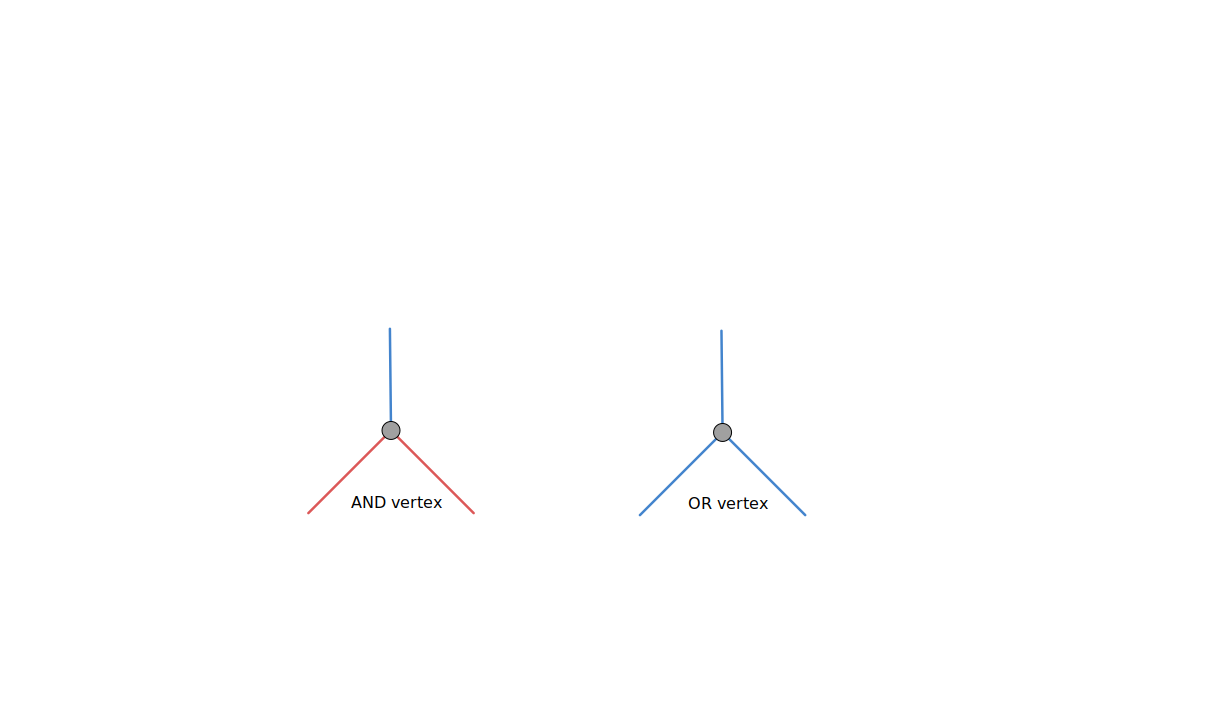
\includegraphics[width=0.35\textwidth]{res/andOrVertex.pdf}
\caption{left image: AND vertex     right image : OR vertex}
\label{fig:circle}
\end{figure}

A vertex with two red edges and one blue edge behaves like an AND gate because it requires both red edges to point inwards before the blue edge can be made to point outwards. 
\begin{figure}[H]
\centering
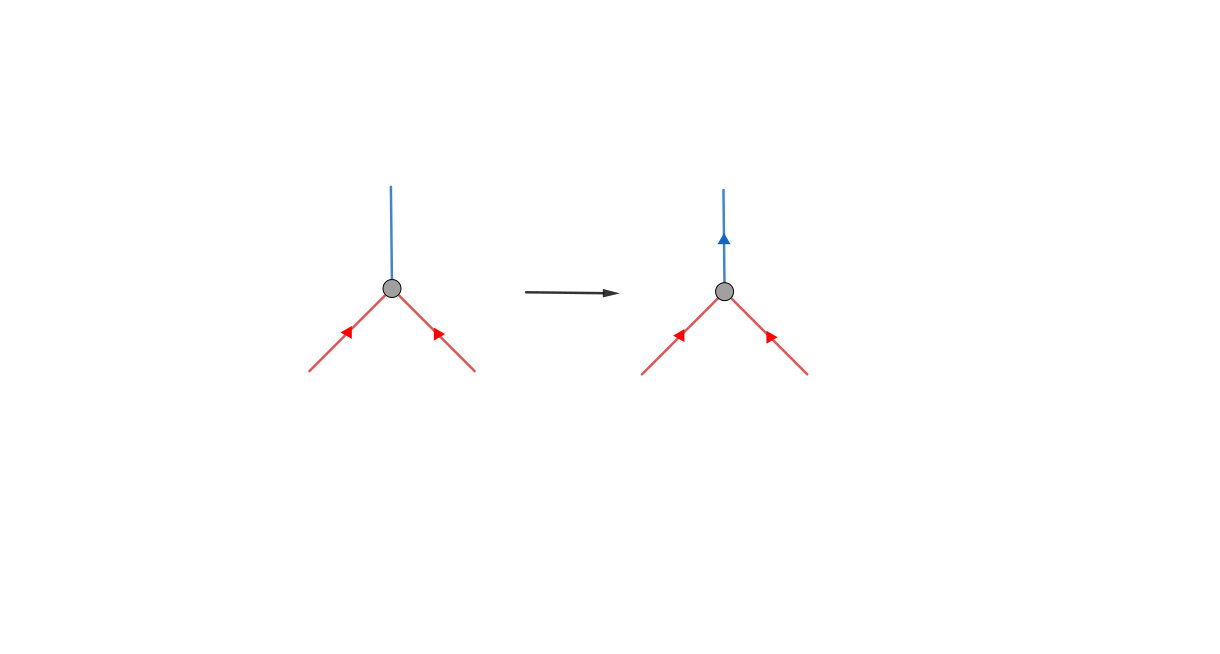
\includegraphics[width=0.35\textwidth]{res/andVertex.pdf}
\caption{Activation of the output edge when the two input edges are activated}
\label{fig:circle}
\end{figure}

A vertex with three blue edges behaves like an OR gate, since it requires at least one input edge to point inwards before the output edge can be activated.
\begin{figure}[H]
\centering
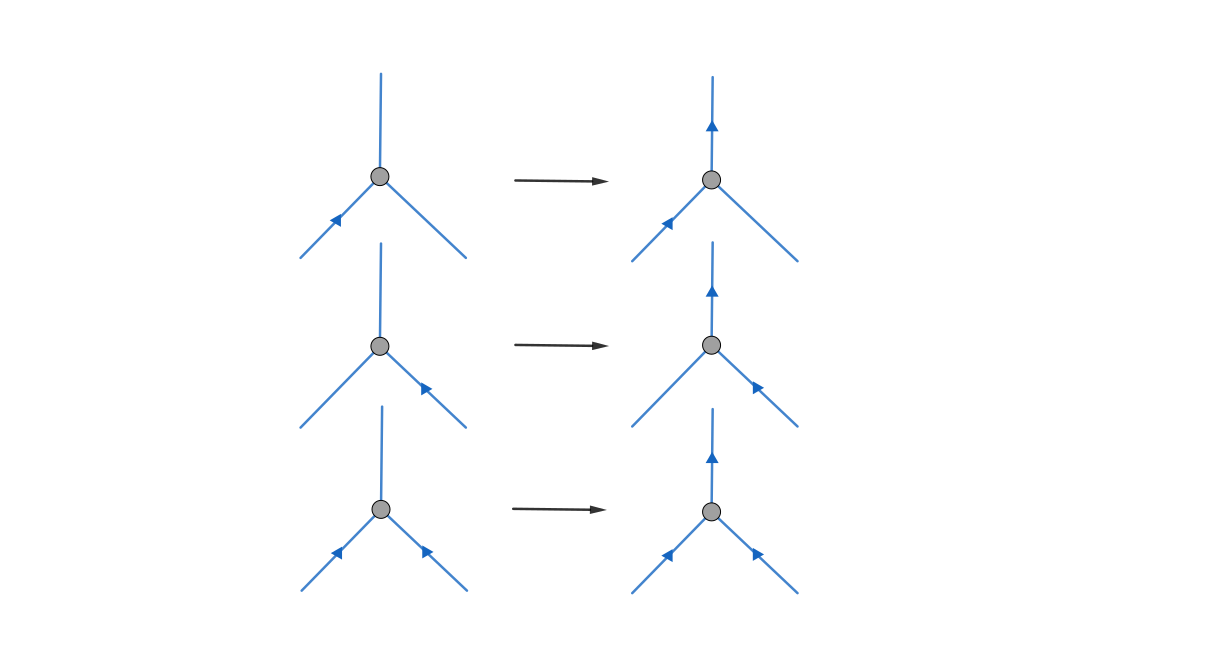
\includegraphics[width=0.35\textwidth]{res/orVertex.pdf}
\caption{Different behaviours of an OR vertex}
\label{fig:circle}
\end{figure}

\begin{defn}
Activation of an edge :  
\begin{enumerate}
    \item An input edge is active when it is an incoming edge. 
    \item An output edge is active when it is an outgoing edge.
\end{enumerate}
\end{defn}

\begin{defn}
Two decision problems arise regarding the graph formulation of the  NCL machine. 
\begin{enumerate}
    \item Given the and/or constraint graph, can a specified edge be eventually reversed by a sequence of reconfiguration steps ?
    \item Given two satisfying configurations, is one configuration reachable to the other by a single edge reversal at a time? 
\end{enumerate}
The answer to both questions happens to be PSPACE-complete. 
In this work a proof sketch is given for the second question.
\end{defn}

\subsection{PSPACE-completeness}

\subsubsection{NCL is PSPACE-hard}
\begin{proof}
The PSPACE-hardness of NCL is proved by doing a reduction from QBF problem, a well known PSPACE-complete problem. The goal of this reduction is to translate a given Quantified Boolean Formula $\phi$ into an instance of NCL so that the result gate in the resulting circuit may be activated if and only if $\phi$ is true. 

\begin{defn}
QBF is the generalized satisfiability problem that includes universal ($\forall$) and existential $(\exists)$ quantifiers. A QBF formula is a Boolean formula containing quantifiers. 
\end{defn}

\paragraph{QBF $\leq_p$ NCL} \hfill \break

\begin{figure}[H]
\centering
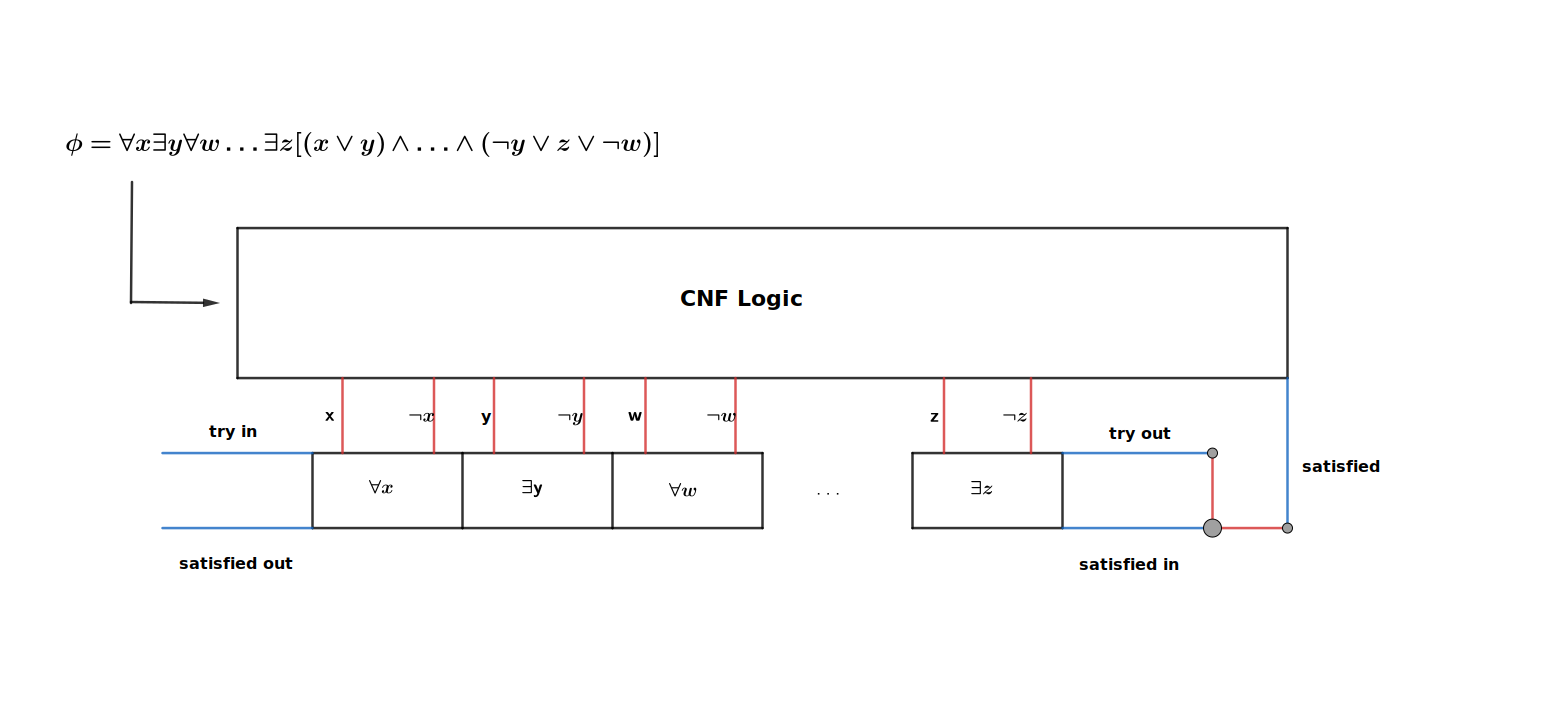
\includegraphics[width=0.9\textwidth]{res/NCL.pdf}
\caption{Schematic of the reduction from Quantified Boolean Formulas to NCL}
\label{fig:circle}
\end{figure}

The reduction from QBF to NCL to prove the PSPACE-hardness is given in the following steps : 
\begin{enumerate}
    \item Compute the and/or constraint graph of the unquantified formula ($[(x \vee y) \wedge \dots \wedge (\neg y \vee z \vee \neg w)]$) which will referred to as the CNF netork. This problem is 
    $\mathcal{NP}-complete$\cite{goos_nondeterministic_2002}.
    \item Associate a quantifier gadget to each quantifier variable in the formula($\forall x \exists y \forall w \dots \exists z$). Each quantifier gadget is connected together.
    \item Associate a variable gadget to represent each variable in the formula. 
    \item Connect each quantifier gadget to its corresponding variable gadget. The orientation of each edge designates which variable is assigned to true or false.  
    \item The variable gadgets are then fed into the CNF network. 
    \item The output of the CNF network is connected to the rightmost quantifier gadget through an AND vertex. 
    \item The output of the overall circuit comes through the satisfied out port from the leftmost quantifier gadget. 
\end{enumerate}

\paragraph{The gadgets in more detail} \hfill \break
\begin{enumerate}
   \item Existential quantifier gadget.
   \begin{figure}[H]
    \centering
    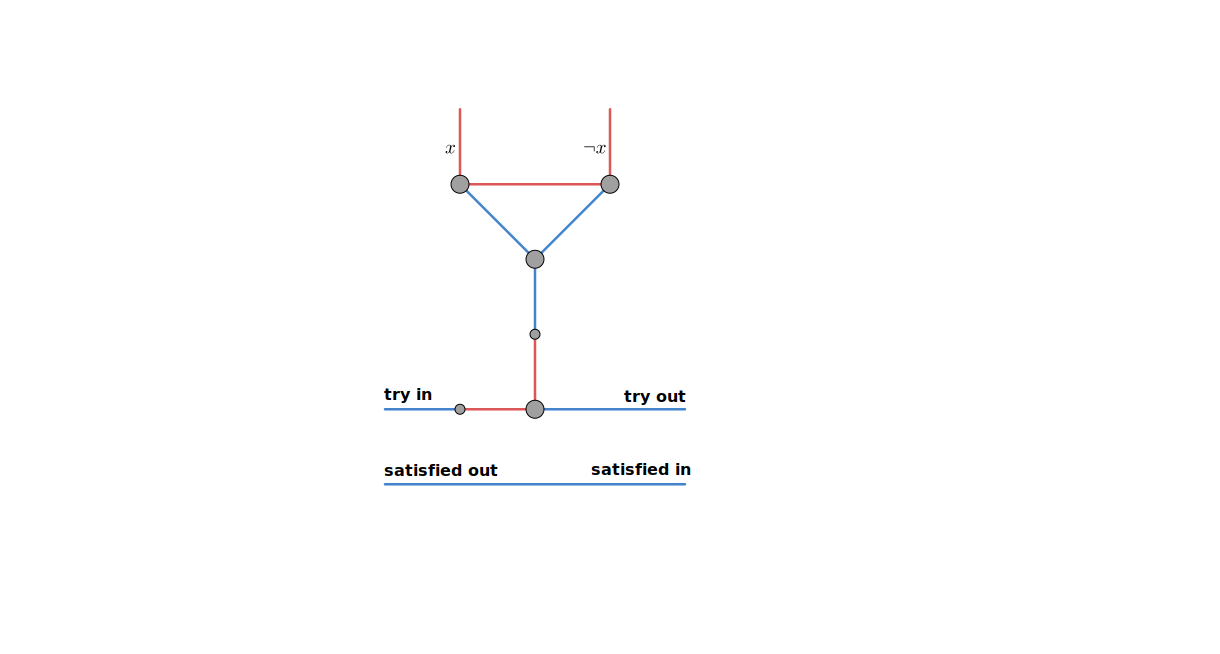
\includegraphics[width=0.3\textwidth]{res/existential.pdf}
    \caption{Existential gadget}
    \label{fig:circle}
    \end{figure}
    
    \begin{enumerate}
        \item The try in edge is considered as the input edge.
        \item The try out edge is considered as the output edge. 
        \item The top part of the existential gadget is called a latch. \\
        The latch is in locked state when its designated output edge is activated. It is called locked state because when the output edge is activated no other edge in the latch can change orientation.
        
        \begin{figure}[H]
        \centering
        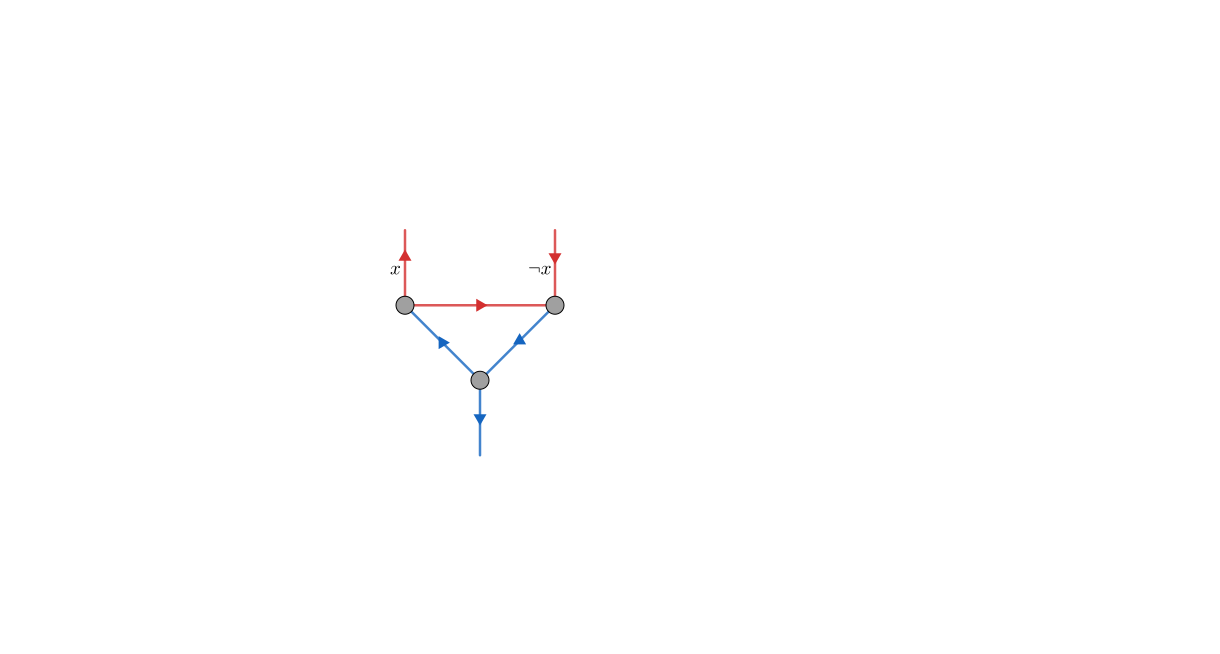
\includegraphics[width=0.2\textwidth]{res/existential2.pdf}
        \caption{Latch}
        \label{fig:circle}
        \end{figure}

        \begin{example}
        If the designated output port is the edge $(1)$ and it points downwards, it prevents other edges from changing orientation. For instance edge $(2)$ cannot flip, which then prevents edges $(3)$ and $(4)$ from reversing. Thus edge $(5)$ cannot point inwards either. Only edge $(6)$ can reverse. 
        
        \begin{figure}[H]
        \centering
        \includegraphics[width=0.2\textwidth]{res/existential3.pdf}
        \caption{Locked state}
        \label{fig:existential3}
        \end{figure}
        \end{example}
        
        \item The latch is then connected to the bottom part of the existential gadget through an edge converter which converts edge $(1)$ from a red edge to a blue edge. (the details about the edge converter gadget is omitted here. Refer to \cite{goos_nondeterministic_2002} for more details). \\
        
        In summary the existential gadget works as follows : 
        It receives a signal from the previous quantifier gadget to assign a value to its variable. Once the variable value is locked, edge ($6$) in figure \ref{fig:existential3} points out, activating the red edge.Thus allowing the try out edge to activate and signal the next quantifier gadget to do the same process. If the later reports back with a positive answer, the current gadget returns the answer back to its caller.  
        
        \begin{figure}[H]
        \centering
        \includegraphics[width=0.3\textwidth]{res/existential1.pdf}
        \caption{Universal quantifier gadget signaled to assign a value to its variable and to signal the next quantifier to do the same}
        \label{fig:circle}
        \end{figure}
    
    \end{enumerate}
    
    \item Universal quantifier gadget. \\ 
    The universal quantifier has a slightly more complex structure than the existential quantifier. 
    There are two latches in the universal gadget. Both whose edges are connected to an AND gate. As earlier the latches play the role of a one bit memory since their locking mechanism allows the assignment of the different variables to true or false. The satisfied out edge is activated only when both latches are in locked in state i.e when the assignments are successful. 
    
    \begin{figure}[H]
    \centering
    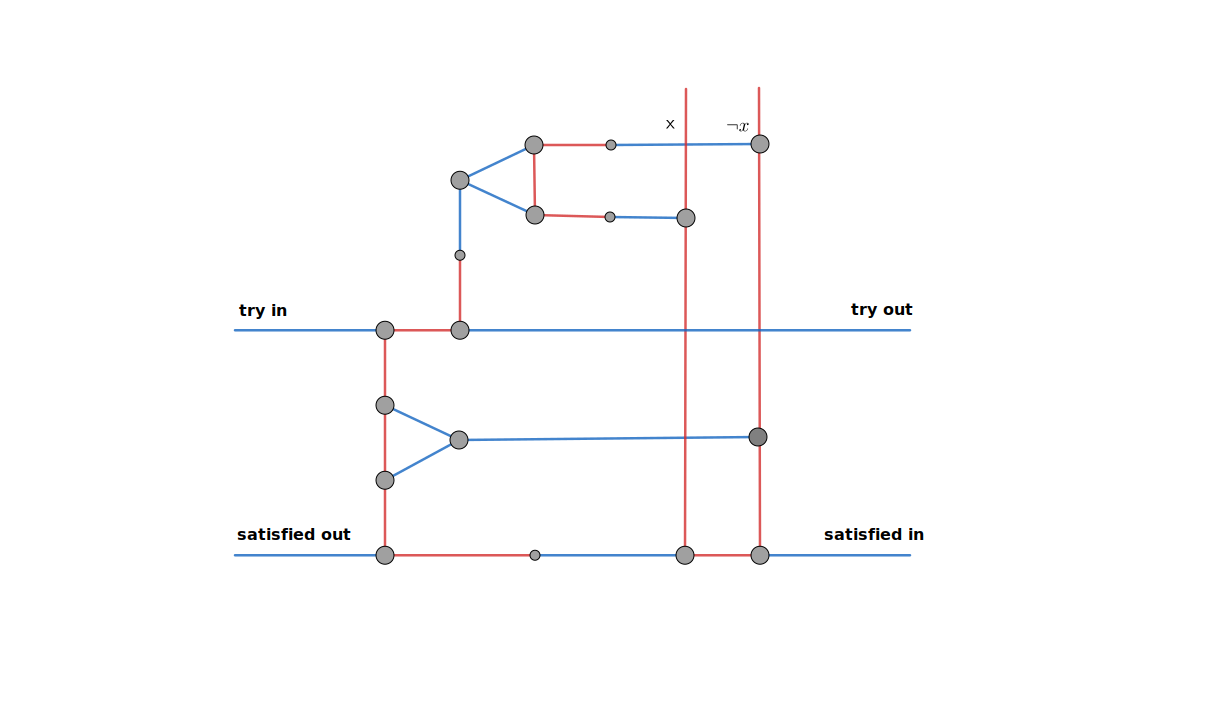
\includegraphics[width=0.7\textwidth]{res/universal.pdf}
    \caption{Universal quantifier gadget}
    \label{fig:circle}
    \end{figure}
    
    \item The variable gadget \\
    The variable gadget is none other than the latches encountered in the universal and existential gadgets.
\end{enumerate}

\paragraph{The general workflow} \hfill \break

Once the CNF network is computed, the result comes through the satisfied edge. The satisfied edge is activated if and only if the CNF formula is satisfied. 
Once all the variables are set, the try out edge is activated as well which then allows edges $(1)$ and $(2)$ to activate leading to the activation of the satisfied in edge. 
   
    \begin{figure}[H]
    \centering
    \includegraphics[width=0.9\textwidth]{res/NCL1.pdf}
    \caption{Schematic of the reduction from Quantified Boolean Formulas to NCL}
    \label{fig:circle}
    \end{figure}
    
This, then activates the quantifier gadgets leading to the activation of the satisfied out edge if and only if $\phi$ is satisfied.   

\begin{lemma}\cite{goos_nondeterministic_2002}
A quantifier gadget${^'}$s satisfied in port may not activate unless its try out port is active.
\end{lemma}

\begin{lemma}\cite{goos_nondeterministic_2002}
An existential quantifier gadget may activate its satisfied out port if and only if its satisfied in port is active with its variable locked in some state.
\end{lemma}

\begin{lemma} \cite{goos_nondeterministic_2002}
A universal quantifier gadget may activate its satisfied out port if and only if its satisfied in port is at one time active with its variable locked in the false (x) state, and at a later time is again active with its variable locked in
the true (x) state, with try in remaining active throughout.
\end{lemma}

\begin{lemma} \cite{goos_nondeterministic_2002}
A quantifier gadget may activate its satisfied out port if and only if its try in port is active, and the formula read from the corresponding quantifier to the right is true given the variable assignments that are fixed by the quantifier
gadgets to the left.
\end{lemma}

\begin{theorem}
NCL is PSPACE-complete
\cite{goos_nondeterministic_2002}
\end{theorem}

\end{proof}
\section{Reconfiguration of satisfiability problems}
\label{sec:SAT}
The focal point of this section is the connectivity-related properties of the solution space of Boolean satisfiability problems with a focus on the complexity of the connectivity and st-connectivity questions defined earlier in section \ref{sec:reconfigureIntro}.

\subsection{SAT}
\begin{defn}The satisfiability problem is to test whether a Boolean formula is satisfiable. SAT = $\{\langle \phi \rangle | \phi$  is a satisfiable Boolean formula$\}$. i.e to decide if an assignment of $0_s$ and $1_s$ to its variables, makes the formula evaluate to true.
\end{defn}

\begin{defn}
A CNF formula is a Boolean formula of the form $C_1 \wedge C_2 \wedge,\dots,\wedge C_m$ where each $C_i$ is a clause. A clause is a disjunction of multiple literals. A literal may be a variable or a negation of a variable.
\end{defn}

\begin{theorem}[Cook-Levin]
SAT is $\mathcal{NP}$-complete.
\end{theorem}

\subsection{Satisfiability reconfiguration problems}
\begin{defn}
Given a boolean formula $\phi$ with $n$ boolean variables $\{x_i,x_{i+1}, \dots, x_n\}$ with $i = \{0,\dots, n\}$ and two configurations $s_0$, $s_t$ from $\{T,F\}^{n}$ that satisfy $\phi$, is there a way to transform one configuration to the other with the following constraints: 
\begin{enumerate}
    \item At each step, only one variable $x_i$ can be flipped.
    \item Each intermediate configuration $x_k$ must be feasible i.e satisfy $\phi$.
\end{enumerate}
\end{defn}

\subsubsection{Configuration graph} 
\begin{defn}
The graph $G = (V,E)$ considered here is an $n$ dimensional hypercube where $V= \{$the collection of all possible assignments$\}$ and $E = \{$collection of edges that links all pairs of vertices that differ exactly in one variable$\}$. 
\end{defn}

\begin{example}
$\phi = (x_1 \vee x_2 \vee \neg x_3) \wedge (x_1 \vee \neg x_2 \vee x_3) \wedge (\neg x_2 \vee \neg x_3 \vee \neg x_1)$ and the two satisfying assignments are : 
$s_0 =(true, false, true) $ and $s_t =(false, true, true)$ i.e $s_0 = (1,0,1)$ and $s_t = (0,1,1)$.  \\

\begin{figure}[H]
\centering
\includegraphics[width=0.8\textwidth]{res/hypercube.png}
\caption{left image:3-dimensional hypercube containing all possible assignments. Right image : two assignments satisfying $\phi$.}
\label{fig:circle}
\end{figure}
\end{example}

\subsubsection{Basic concepts and statements of results}
The first to analyze the connectivity properties of the configuration graphs of satisfiability problems were Gopalan et al. \cite{gopalan_connectivity_2006}. Their work is the continuity of Schaefer's work \cite{schaefer_complexity_1978}. The latter introduced a framework for expressing variants of Boolean satisfiability and a very well celebrated theorem called the Dichotomy theorem. 

\paragraph{Schaefer's framework}
\begin{defn}
A logical relation $\mathcal{R}$ is a non-empty subset of $\{T,F\}^{k}$ where $k$ is the arity of $\mathcal{R}$ for some $k \geq 1$. 

\begin{example}
If $\mathcal{R}_{1/3} = \{TFF,FTF,FFT\}$, then  $\mathcal{R}_{1/3}(x_1,x_2,x_3)$ is TRUE if and only if exactly one of $x_1$,$x_2$,$x_3$ is assigned to TRUE. 
\end{example}
\end{defn}

\begin{defn}
Let $\mathcal{S}$ be a finite set of logical relations. A  $CNF(\mathcal{S})-formula$ over a set of variables $V = \{x_1,x_2,\dots,x_n   \}$  is a finite conjunction $c_1 \wedge c_2 \wedge \dots \wedge c_m$ of clauses built using relations from $\mathcal{S}$. \\
Hence each $c_i$ is an expression of the form $\mathcal{R}(\varepsilon_1,\varepsilon_2,\dots,\varepsilon_k)$ where $\mathcal{R}$ is a logical relation and each $\varepsilon_j \in V or \{T,F\}$. A solution of a $CNF(\mathcal{S})-formula$ $\phi$ is an assignment $s = (s_1, \dots, a_n)$ of Boolean values to the variables that makes every clause of $\phi$ true. 
\end{defn}

\begin{defn}
The $SAT(\mathcal{S})$ problem associated with a finite set of logical relations $\mathcal{S}$ asks : 
Given a CNF($\mathcal{S}$)-formula $\phi$, is it satisfiable ?
\end{defn}

\begin{remark}
All well known restrictions of Boolean satisfiability problems, such as $3$-SAT, NOT-ALL-EQUAL $3$-SAT and POSITIVE $1$-IN-$3$SAT can be cast as SAT($\mathcal{S}$) problems, for a suitable choice of $\mathcal{S}$. 
\end{remark}

\begin{example}
Let $R_0 = \{0,1\}^{3} \backslash \{000\}$,
$R_1 = \{0, 1\}^{3} \backslash\{100\}$, $R_2 = \{0,1\}^{3} \backslash\{110\}$, $R_3 = \{0,1\}^{3} \backslash\{111\}$. Then $3-SAT$ is the $SAT(\mathcal{S})$ problem where $\mathcal{S} =   ({R_0 , R_1 , R_2 , R_3 })$. Similarly, POSITIVE 1- IN -3S AT is $SAT({R_{1/3}})$, where $R_{1/3} = \{100, 010, 001\}$.
\end{example}

\paragraph{Dichotomy theorem} \\ [breakline]
\\
Schaefer classified the Boolean constraint satisfaction problem and showed that, for certain sets $\mathcal{S}$, $SAT(\mathcal{S})$ is solvable in polynomial time while for all other sets $\mathcal{S}$ the problem is $\mathcal{NP}-complete$. \\ 
Schaefer gave $6$ classes for which $SAT(\mathcal{S})$ is solvable in polynomial and proved that all other sets of relations generate an $\mathcal{NP}$-complete problem. \\ 
A set $\mathcal{S}$ of logical relations is Schaefer if all relations in $\mathcal{S}$ are either bijunctive, Horn, dual Horn, or affine. \cite{schaefer_complexity_1978}

\paragraph{Tight relations class\cite{gopalan_connectivity_2006}}
The class of tight relations can be seen as a superset of Schaefer relations. Gopalan et al. were mostly interested about the reachability problem and thus created a dichotomy theorem analogous to Schaefer's.  

\begin{defn}
st-Conn($\mathcal{S}$) : Given a CNF($\mathcal{S}$)-formula $\phi$, and two satisfying assignments $s$ and $t$ of $\phi$,is there a path between $s$ and $t$ in the configuration graph of solutions of $\phi$?
\end{defn}

\begin{defn}
Conn($\mathcal{S}$)Given a CNF($\mathcal{S}$)-formula $\phi$, is the configuration graph of solutions of $\phi$ connected?
\end{defn}

\begin{theorem} \cite{DBLP:journals/corr/Heuvel13}
Let $\mathcal{S}$ be a finite set of logical relations.
\begin{enumerate}
    \item If $\mathcal{S}$ is tight, then st-Conn($\mathcal{S}$) is in $\mathcal{P}$; \\otherwise, st-Conn($\mathcal{S}$) is PSPACE-complete. 
    \item If $\mathcal{S}$ is tight, then Conn($\mathcal{S}$) is in coNP, \\if it is tight but not Schaefer, then it is coNP-complete; \\otherwise, it is PSPACE-complete.
    \item If every relation R in S is the set of solutions of a 2-CNF-formula, then
Conn(S) is in P.
\end{enumerate}
\end{theorem}

\begin{footnotesize}
Please refer to \cite{gopalan_connectivity_2006} for the formal definition of tight sets 
\end{footnotesize}



\section{Binary Integer programming Reconfiguration problems}
\label{sec:BIP}
\subsection{Integer programming}
\begin{defn}
An integer programming problem is defined as a mathematical optimization
problem where the objective function and the constraints must be integers. 
More formally it is defined as follows :
\begin{center}
    \begin{maxi!}|l|
	  {x}{cx : Ax \leq b, x \in \mathbb{Z}^{n}}{}{}
    \end{maxi!}
\end{center}
where $A$ is an $m\timesn$ integer matrix, $c$ an $n-$dimensional row vector, $b$ an $m-$dimensional column vector and $x$ an $n-$dimensional column vector of variables or unknowns. 
\end{defn}

\begin{defn}
A binary integer programming problem also known as $0-1$ integer programming problem is an integer programming problem where $x \in \{0,1\}^{n}$. 
\end{defn}

\begin{defn}
The set of solution to the BIP is the set of vectors $V$ that satisfy all the constraints. The set $V$ is also called the set of feasible solutions. 
\end{defn}

\subsubsection{Geometry of integer programming}
\begin{defn}
Each constraint in an integer programming problem can be transformed into an equation which then represents a hyperplane in $\mathbb{R}^{n}$, a plane in $\mathbb{R}^{3}$ and a line in $\mathbb{R}^{2}$ and a point in $\mathbb{R}^{1}$ .
\end{defn}

\begin{defn}
The inequation represents one of two half spaces, which is the solution set of the inequations. A halfspace in $\mathbb{R}^{n}$ is a set of the form $\{x \in \mathbb{R}^{n} : a^{T}x \leq b\}$ for some vector a $\in$ $\mathbb{R}^{n}$ and $b \in R$.
\end{defn}

\begin{defn}
A polyhedron is the intersection of finitely many halfspaces: $P = \{x \in \mathbb{R}^{n} : Ax \leq b\}$ with edges as lines, planes, hyperplanes as the case may be.
\end{defn}

\begin{defn}
A polytope is a bounded polyhedron.
\end{defn}
\begin{example}
    \begin{maxi!}|l|
	  {}{Z = 8x_1 - 7x_2}{}{}
    \end{maxi!}
subject to : 
\begin{gather}
    x_1 + x_2 \leq 5 \\
    4x_1 + 7x_2 \leq 28 \\
    2x_1 - 3x_2 \leq 6 \\
    -3x_1 + 4x_2 \leq  12 \\
    x_1 \geq 0, x_2 \geq 0
\end{gather}
\end{example}

    \begin{figure}[H]
    \centering
    \includegraphics[width=1.0\textwidth]{res/integerp.pdf}
    \caption{Polytope yielded by the constraints of the optimization problem where the solution points correspond to the lattice points.}
    \label{fig:circle}
    \end{figure}

\subsubsection{Complexity}
\begin{theorem}
The $0-1$ integer programming problem is $\mathcal{NP}-$complete.
\end{theorem}

\begin{proof}
To prove that $0-1$ integer programming problem is $\mathcal{NP}-$complete. The two following conditions have to be satisfied : 
\begin{enumerate}
    \item $0-1$ integer programming problem is in $\mathcal{NP}$.
    \item Any problem $B$ in $\mathcal{NP}$ $\leq_{p}$ $0-1$ integer programming
    problem.\\
    The second condition can be proved by the reduction from a known $\mathcal{NP-}$complete problem.
\end{enumerate}

\paragraph{The $0-1$ integer programming problem is in $\mathcal{NP}$}.  \hfill \break
To prove that $0-1$ integer programming is in $\mathcal{NP}$ a straightforward polynomial time algorithm deciding it, is the following :  \\ 
\\
$M = $``On input $(A, b, x)$\\
1. multiply matrix $A$ with vector $x$\\
2. for $i \in (1,\ldots,m)$\\
3. ~ if $(Ax)_i > b_i$ reject\\
4. accept 

\begin{enumerate}
    \item  Multiplying each component of a row of $A$ with each component of $x$ and doing this for $m$ rows of $A$ takes $m\cdot O(n) = O(m \cdot n )$ time. 
    \item  Comparing component wise each element of $(Ax)$ with each element of $b$ makes in total $m$ comparisons is $O(m)$. 
\end{enumerate}
Final time complexity is $O(m \cdot n) + O(m) = O(m \cdot n)$ which means that $0-1$ integer programming $\in \mathcal{NP}$.

\begin{defn}
A cnf-formula is a $3$cnf-formula if all its clauses has $3$ litterals. For example  
$\phi = (x_1 \vee x_2 \vee \neg x_3) \wedge (\neg x_1 \vee x_2 \vee x_3)$. $3SAT = \{\langle \phi \rangle | \phi$  is a satisfiable Boolean formula$\} $
\end{defn}

\begin{theorem}
$3$SAT is $\mathcal{NP}$-complete.
\end{theorem}

\paragraph{$3$SAT $\leq_{p}$ $0-1$ integer programming} \hfill \break
Let $\phi$ be a $3SAT$ formula with $m$ clauses and $n$ variables. The binary integer programming instance will be constructed in the following way :  \hfill \break

For each clause in the $3SAT$ instance, we create the constraint that the sum of literals, using $z_i$ to represent $x_i$ and $(1-z_i)$ to represent $\neg x_i$, is at least 1. 
For example if $\phi=$ $(x_1 \vee \neg x_2 \vee x_3)$, the BIP instance will be constructed  as following : $z_1 + (1-z_2) + z_3 \geq 1$.  \hfill \break

To satisfy this inequality either $z_1$ should be set to $1$ or $z_2=0$ or $z_3=1$, which means we either set $x_1=true$ or $x_2=false$ or $x_3=true$ in the corresponding truth assignment.  \hfill \break

We can easily check that this construction works. \hfill \break
\begin{enumerate}
    \item Assuming that we have a satisfying assignment $S$ for $\phi$. After the construction, since $S$ is a satisfying assignment, at least one literal in each clause must be satisfied. Therefore the associated sum corresponding to constraints in the BIP instance is $\geq 1$.
    \item In the other direction, we assume we have a feasible solution to the BIP. Hence it means that each inequality must be satisfied i.e be $\geq 1$. This implies that at least one of the corresponding literal is set to $1$, since each inequality is the sum of three variables set to $1$ or $0$.
\end{enumerate}

\end{proof}

\subsection{Constrained Hypercube Path} 
The constrained hypercube path can be seen as a reconfiguration analogue to the $0-1$ Integer programming problem defined above. It is defined as follows : 

\begin{defn} \cite{cardinal_reconfiguration_2018}
Given two vertices $s,t$ of the $n-hypercube$ both be contained in a polytope $P := \{x \in \mathbb{R}^{n} : Ax \leq b\}$ for $A \in \mathbb{Z}^{d \times n}$ and $b \in \mathbb{Z}^{d}$, is there a path from $s$ to $t$ in the hypercube such that each vertices of the intermediate solution lies in $\mathcal{P}$
\end{defn}

\begin{example}
\end{example}
\begin{figure}[!h]
  \centering
  \def\svgscale{0.5}
   \def\svgwidth{width = 0.2}
  \includesvg{res/3d}
  \caption{$3$-hypercube solution space where the constraints are planes}
\end{figure}

\begin{theorem}
The constrained hypercube path problem is PSAPCE-complete, even when $d = O(1)$. \cite{cardinal_reconfiguration_2018}
\end{theorem}

\begin{proof}
The above theorem is proved by a reduction from a variant of the exact cover reconfiguration problem. It is the exact cover reconfiguration problem where more-than-2-way merges and splits are permitted. 

\begin{defn}
Exact cover problem : Given a collection $S$ of subsets of set $X$, an exact cover is the subset $S^{*}$ of $S$ such that each element of $X$ is contained is exactly one subset of $S^{*}$. It should satisfy the following two conditions : 

\begin{enumerate}
    \item The intersection of any two subsets in $S^{*}$ should be empty. That is, each element of $X$ should be contained in at most one subset of $S^{*}$.
    \item Union of all subsets in $S^{*}$ is $X$. That means union should contain all the elements in set $X$. So we can say that $S^{*}$ covers $X$.
\end{enumerate}
The Exact cover problem is a decision problem to determine if exact cover exists or not. 
\end{defn}
\begin{example}
Let $S = \{A, B, C, D, E, F\}$ and $X = \{1, 2, 3, 4, 5, 6, 7\}$ such that :\\ 
$A = \{1, 4, 7\}$ \\
$B = \{1, 4\}$ \\
$C = \{4, 5, 7\}$ \\
$D = \{3, 5, 6\}$ \\
$E = \{2, 3, 6, 7\}$ \\
$F = \{2, 7\}$ \\
Then $S^* = \{B, D, F\}$ is an exact cover, because each element in $X$ is contained exactly once in subsets $\{B, D, F\}$ . If we union subsets then we will get all the elements of $X$ – $B \cup D \cup F = \{ 1,2,3,4,5,6,7\}$
\end{example}

\begin{defn}
Exact cover reconfiguration problem : Given a collection $S$ of subsets of a set $X$ and two exact covers $C_1$ and $C_2$, can $C_1$ be reconfigured into $C_2$ via repeated splits and merges? 
\end{defn}

\begin{defn}
We could also transform an instance of the exact cover problem as a hypergraph $G = (X, S)$ where $X$ is a set and $S$ is a collection of subsets of $X$. The vertices of $G$ would be each element of $X$ and each element of $S$ is a hyperedge. 
We say that a hypergraph is $k$-colorable whenever we can assign one of $k$ colors to each vertex such that no two vertices in a hyperedge have the same color.

\end{defn}

\begin{lemma}
The exact cover reconfiguration problem is PSPACE-hard for instances that are $23$-colorable hypergraphs. \cite{cardinal_reconfiguration_2018}
\end{lemma}

\end{proof}

\section{Open questions}
\begin{enumerate}
    
    \item What is the connection between the complexity of reconfiguration problems and the complexity of the decision problem on the existence of configurations of a particular kind ? 
    
    \item What properties of problems result in the pattern holding or
    not? Related to the exceptions discussed in section \ref{sec:reconfigureIntro}
    
    \item It is possible to refine Gopalan et al.'s dichotomy even more ? 
    \item (Related to the constrained hypercube path problems) Is the traveling salesman reconfiguration problem (where two tours are adjacent if they differ in two edges) PSPACE-complete?

\end{enumerate}


\newpage
\nocite{*}
\bibliographystyle{alpha}
\bibliography{main}

\end{document}
